\subsection{Partial SPIDER}
The \textit{SPIDER} Algorithm \cite{bauckmann2006efficiently} was devised for unary IND discovery, employing an all-column sort merge join technique. It operates in two main phases. Initially, it sorts each attribute and stores the sorted values in one file per attribute. Subsequently, it conducts a $k$-way merge while simultaneously validating the candidates.

To extend the \textit{SPIDER} algorithm for partial IND discovery, it becomes essential to monitor the frequency of each value alongside the total count of unique values. Bauckmann et al. have already proposed an adjusted algorithm capable of partial IND discovery. Their suggestion involves integrating a counter to monitor violations, invalidating candidates when the violation count exceeds a threshold. This approach is effective when duplicates are disregarded. Should the duplication distribution be of concern, the authors suggest retrieving such information from a database, as values are deduplicated during sorting. While this is valid, it remains unclear how occurrences are managed thereafter. Assuming the occurrences of all values surpass the capacity of main memory, querying the database for each value could becomes necessary, which presents a massive computational overhead. We will propose a partial version of \textit{SPINDER} called \textit{pSPIDER} which is capable of finding partial unary INDs in the \textit{duplicateAware} and \textit{duplicateUnaware} setting using a unified procedure.

\subsubsection{\textbf{Existing Code.}}
The authors of \textit{SPIDER} did not provide a linkage to the source code used for the experiments. For the work conducted by Dürsch et al. on the comparison of multiple IND discovery algorithms\cite{dursch2019inclusion}, they published an implementation of \textit{SPIDER} through GitHub\footnote{\href{https://github.com/HPI-Information-Systems/inclusion-dependency-algorithms}{github.com/HPI-Information-Systems/inclusion-dependency-algorithms}}. This implementation will be referred to as the \textit{SPIDER} implementation and is treated as a point of reference when evaluating execution times. Related researched has already shown that there is open potential to increase the performance of \textit{SPIDER}. It has been shown, that by discussing the underlying data structures in detail and moving to a C++ based implementation \cite{smirnov2023fast} a speed-up of up to 5 times is possible. Memory efficient value storing and a changed approach on value sorting where the most influential factors. Instead of sorting during reading, as the Metanome implementation does it, they read the values to vectors and utilize sorting these vectors in parallel once the main memory filled up or the end of the input is reached instead. Similar to Smirnov et al. we will also utilize parallelization and lazy sorting to archive a speed up of ?x? over \textit{SPIDER}.

\subsubsection{\textbf{Sorting Adjustments}}
The \textit{SPIDER} implementation uses a \textit{SortedSet} as its key structure during the attribute sorting. Every value is put into the \textit{SortedSet} in the order of its occurrence. If at some point, the main memory of the executing machine surpasses a set threshold, the values a written to disk. This process is called spilling. We save the sorted subset of values contained in the attribute to disk and release the data from main memory. When all attributes have been sorted we merge the sorted chunks together. Choosing a \textit{SortedSet} holds the advantages, that the values are guaranteed to be sorted at all times, which means spilling value to disk in a sorted manner is trivial. Insertion, deletion or containment checks all have a logarithmic complexity to the number of currently contained elements. Internally, a self balancing red-black is used to guarantee the operation complexity regardless of the value distribution the contained elements posses. A further advantage is, that a \textit{SortedSet} already deduplicates the values, which yields a unique set of keys to which we can add the counts during reading with very little overhead.

While this seems to be the perfect structure, experimental results have shown much room for improvement. We found that lazy sorting in combination with a hash based deduplication is much more efficient. Using a fixed-size HashMap we deduplicate entries and keep track of occurrences using $O(1)$ operations. If the fixed size is reached we sort the entry set of the map by keys and then spill to disk.

To accommodate the occurrences of all values, we have decided to structure the sorted files by writing the value in one line and the number of occurrences in the directly following line. This format is easy to parse and does not required additional string operations like a two column encoding would. Merging sorted files together follows the know strategies of Bauckmann et al.


\subsubsection{\textbf{Validation Adjustments.}}
Before the validation begins, we are aware of the number of unique and total values of every attribute. This information is used to calculate the threshold of violations based on the degree partial degree $\rho$. In a \textit{duplicateAware} setting the number of violations is
$$
violations = \lfloor \frac{\rho \cdot \# unique}{\#unique} \rfloor
$$
while in the \textit{duplicateUnaware} setting we find
$$
violations = \lfloor \frac{\rho \cdot \# total}{\#total}\rfloor.
$$

The validation of \textit{pSPIDER} and \textit{SPIDER} are practically equal. The only difference begin, that \textit{pSPIDER} checks if the number of violations has surpassed a threshold while \textit{SPIDER} prunes immediately once the first violation occurred. When we execute \textit{pSPIDER} in a \textit{duplicateAware} setting each violation decreases the number of open violations by 1 while in the \textit{duplicateUnaware} setting we decrease the open amount by the number of occurrences of the violating value.

\subsubsection{\textbf{Parallelizing pSPIDER}}
We were able to archive a substantial improvement in runtime by parallelizing sorting. To best utilize the parallel capabilities we first split all relations into one file per attribute, which we also parallelize on a relation level. Afterwards, we sort the attributes using all available cores and heuristically start with the most complex attributes. The complexity of sorting is judge by the number of total values, which is counted while splitting the relations. Processing the jobs in an order which minimizes the longest span is an NP-hard problem \cite{graham1979optimization}. However the greedy strategy of always processing the heuristically longest unprocessed job once a tread becomes available (LPT), has been proven robust in both the average and worst case. Due to those results and the simplicity of the approach we will conduct an LPT scheduling. To understand the effectiveness of paralyzing \textit{pSPIDER} Figure \ref{fig:parallel_spider} displays the decrease in the total execution time for all datasets. Each line represents a single dataset, the y-Axis is scaled relative to the execution time of a single thread, the x-Axis represents the parallelization degree. The experiments have been executed on a ?CPU? with ?RAM? GB of main memory and a single ?SSD?. Every setting was computed five time and the times where than averaged to mitigate external factors. While the effective nice of adding more core decreases, we still find a steady decrease in runtime. Our final version therefore tries to utilize as many threads as the machine offers.

\begin{figure}
    \centering
    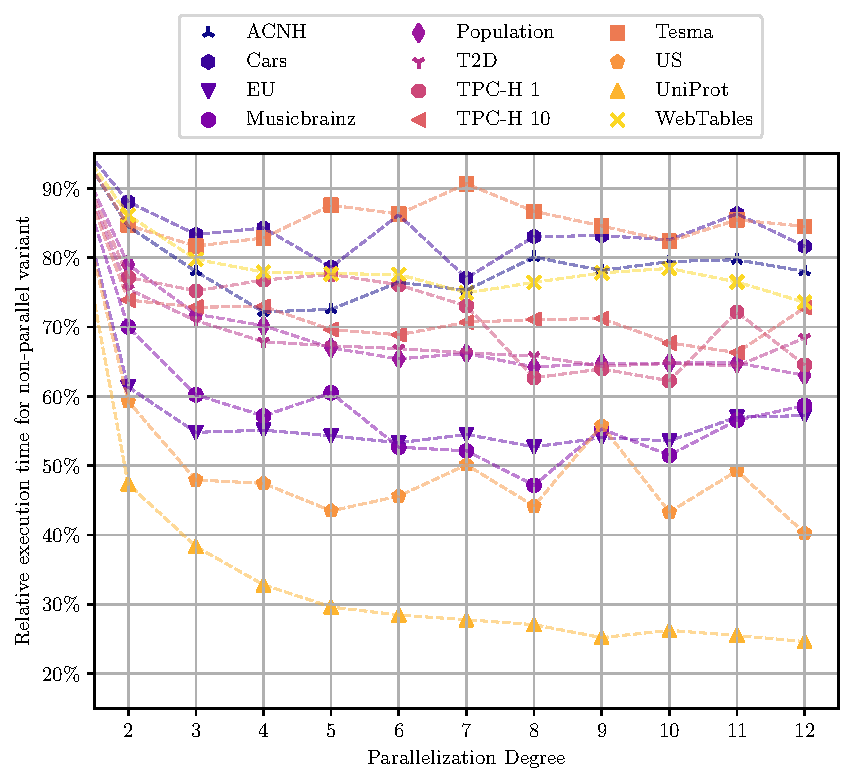
\includegraphics[width=0.475\textwidth]{figures/spider_parallel.pdf}
    \caption{Parallelization effectiveness for \textit{pSPIDER} over various datasets.}
    \label{fig:parallel_spider}
\end{figure}